\section{土日に実施できる確率}
\label{sec:weekend}

打ち上げは土日に行うことが多い。そこで、実施できる日が土日に当たる確率を、
2016--2025 年の実際の暦（曜日・祝日）に日ごとの確率を当てはめて数えた。

\subsection{数え方}

\begin{itemize}
  \item \textbf{土日の 1 日}: 土曜または日曜の 1 日を選んだとき、その日に実施できる確率。
  \item \textbf{決めた土曜}: 何か月も前に「この土曜」と決めた場合の確率。
  \item \textbf{土日のどちらか}: 1 回の週末（土・日の 2 日）のうち、どちらかの日に実施できる確率。
    両日とも挑戦できる前提。
  \item \textbf{土曜に実施できたとき日曜も}: 天気は続くので、土曜と日曜は独立ではない。
    この値が「土日の 1 日」より高ければ、良い日はまとまって来る。
  \item \textbf{1 冬に実施できる土日}: 12--2 月の約 26 日の土日のうち、実施できる日数の期待値。
  \item \textbf{毎週末挑戦して $N$ 週以内}: ある週末から毎週末（土日の両日）挑戦したとき、
    $N$ 回目の週末までに実施できる確率。12--2 月のどの週末から始めても同じ重みで数え、
    2 月末で打ち切った。
\end{itemize}

飛行条件のばらつきによる成否は日ごとに独立な乱数で決めた。天気そのものは実際の日の
並びをそのまま使っているので、悪天候が何日も続く効果は入っている。

\begin{table}[htbp]
\centering
\scriptsize
\caption{土日の確率。上が標準の飛行、下が短時間の飛行。}
\label{tab:weekend}
\resizebox{\linewidth}{!}{\begin{tabular}{llrrrrrrr}
\toprule
飛行 & 候補地 & 土日の & 決めた土曜 & 土日の & 土曜に実施 & 1 冬に実施 & \multicolumn{2}{c}{毎週末挑戦して} \\
& & 1 日 [\%] & 1 日 [\%] & どちらか [\%] & できたとき & できる土日 & 2 週以内 & 4 週以内 \\
& & & & & 日曜も [\%] & [日] & [\%] & [\%] \\
\midrule
標準 & 壱岐（島の中央） & 30 & 34 & 49 & 38 & 7.8 & 71 & 88 \\
標準 & 平戸・大島 & 33 & 36 & 53 & 37 & 8.5 & 73 & 90 \\
標準 & 唐津・加唐島 & 35 & 38 & 54 & 40 & 8.8 & 74 & 91 \\
標準 & 下関・蓋井島 & 33 & 38 & 54 & 37 & 8.6 & 77 & 91 \\
標準 & 山口・徳地 & 35 & 36 & 55 & 42 & 9.0 & 78 & 92 \\
標準 & 糸島・志摩 & 28 & 28 & 45 & 39 & 7.0 & 63 & 82 \\
標準 & 福津 & 25 & 25 & 40 & 37 & 6.1 & 58 & 78 \\
標準 & 廿日市 & 32 & 34 & 51 & 41 & 8.3 & 72 & 88 \\
\midrule
短時間 & 壱岐（島の中央） & 38 & 44 & 60 & 40 & 10.0 & 86 & 97 \\
短時間 & 平戸・大島 & 34 & 38 & 54 & 36 & 8.7 & 75 & 90 \\
短時間 & 唐津・加唐島 & 46 & 50 & 69 & 45 & 12.2 & 90 & 97 \\
短時間 & 下関・蓋井島 & 35 & 37 & 56 & 42 & 9.5 & 82 & 93 \\
短時間 & 山口・徳地 & 38 & 41 & 59 & 46 & 10.2 & 85 & 96 \\
短時間 & 糸島・志摩 & 48 & 51 & 70 & 52 & 12.3 & 89 & 98 \\
短時間 & 福津 & 45 & 46 & 65 & 54 & 11.5 & 85 & 96 \\
短時間 & 廿日市 & 47 & 52 & 67 & 52 & 12.3 & 90 & 98 \\
\bottomrule
\end{tabular}
}
\end{table}

\subsection{結果}

曜日によって天気が変わるわけではないので、「土日の 1 日」は全日の確率とほぼ同じになる。
以下は全地点を同じ方法（地上気象は ERA5）で比べた値である。壱岐のアメダスによる値は
表~\ref{tab:ikiweekend} にある。

壱岐（標準の飛行、ERA5）では、土日の 1 日で \SI{30}{\percent}、1 回の週末のどちらかで
\SI{49}{\percent} である。土曜に実施できた週末に日曜も実施できる確率は \SI{38}{\percent} で、
1 日の確率（\SI{30}{\percent}）より高い。良い日は 2 日続きやすい。

1 冬の 12--2 月に、壱岐で実施できる土日は平均 7.8 日ある。毎週末挑戦すると、
2 週以内に \SI{71}{\percent}、4 週以内に \SI{88}{\percent} の確率で実施できる。
短時間の飛行にすると 2 週以内が \SI{86}{\percent}、4 週以内が \SI{97}{\percent} に上がる。

\textbf{日程を 1 日に固定すると約 3 割、週末の 2 日にしても約 5 割にとどまる}。
予備日として同じ週末の 2 日と、その後の 2--3 週末を確保しておくのが現実的である。

\begin{figure}[htbp]
\centering
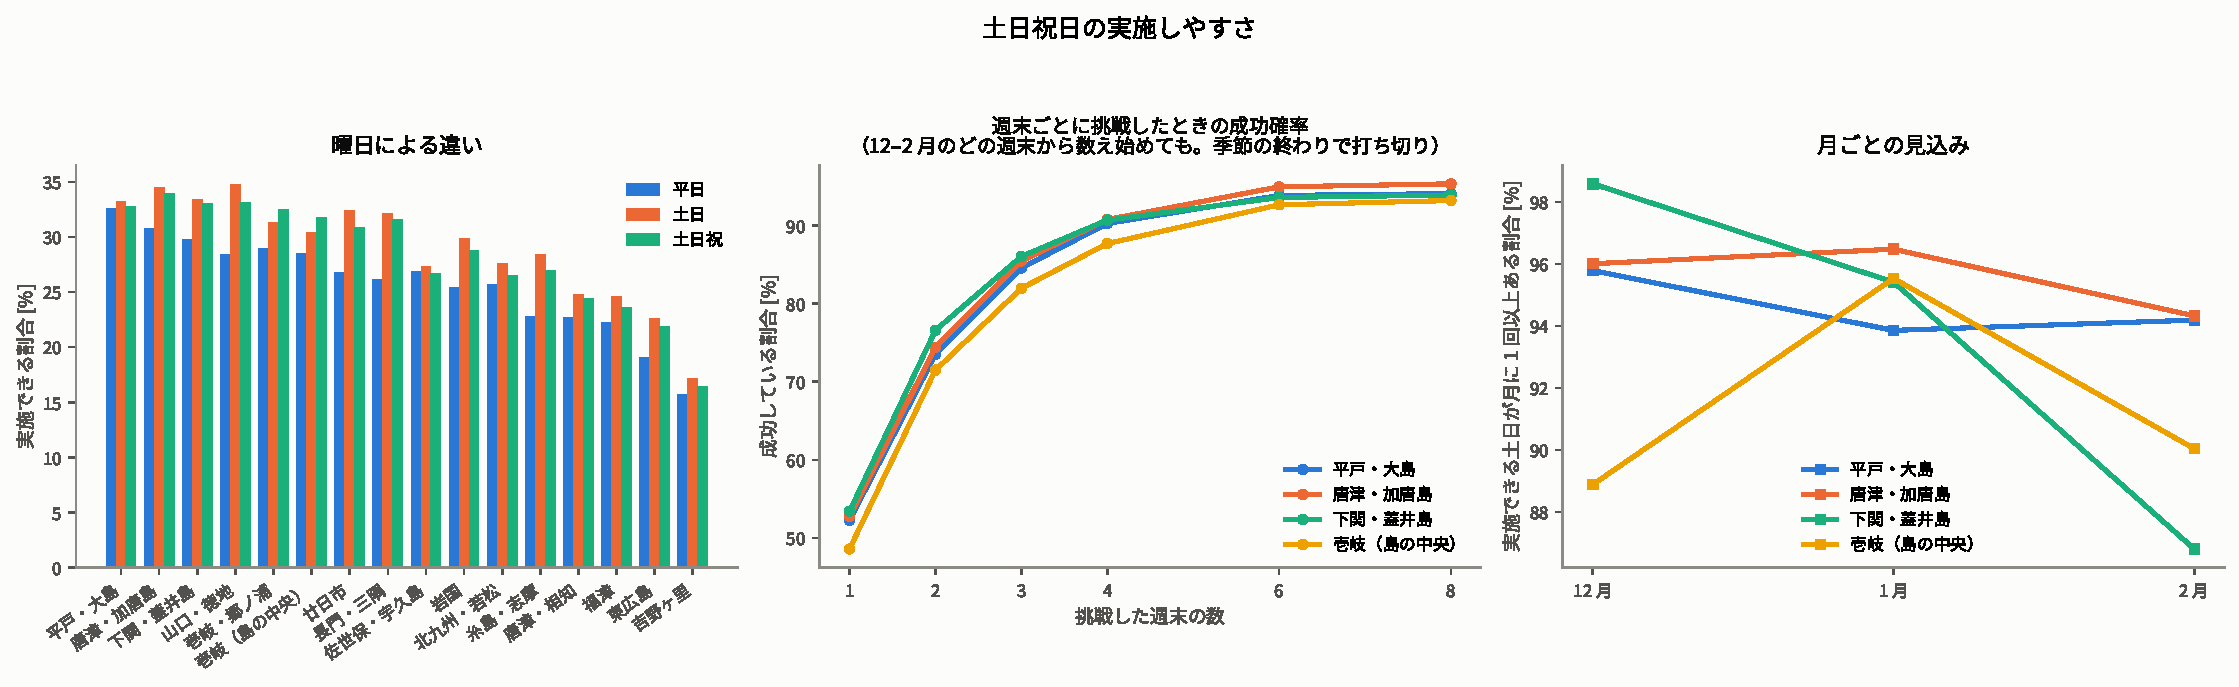
\includegraphics[width=\linewidth]{weekend.pdf}
\caption{土日の確率。(a) 平日・土日・土日祝の 1 日あたりの確率。(b) 毎週末挑戦したとき、
$N$ 回目の週末までに実施できる確率。(c) 各月に実施できる土日が 1 日以上ある確率。}
\label{fig:weekend}
\end{figure}

\begin{figure}[htbp]
\centering
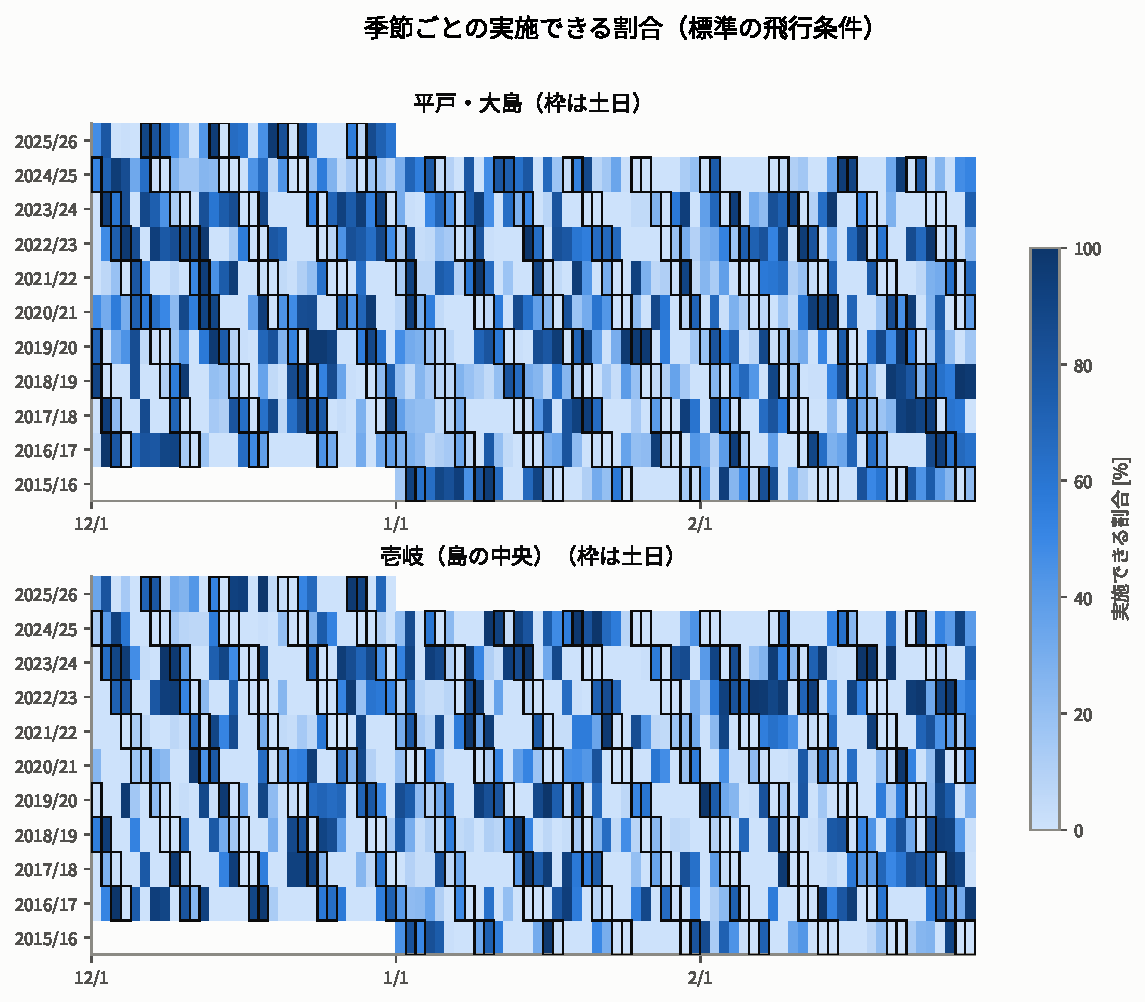
\includegraphics[width=\linewidth]{calendar.pdf}
\caption{日ごとの実施できる確率（標準の飛行）。行が冬（12 月〜翌 2 月）、列が日付。
印は土日。良い日と悪い日がそれぞれ数日ずつかたまって現れる。}
\label{fig:calendar}
\end{figure}

\subsection{月と年による違い}

\begin{table}[htbp]
\centering
\scriptsize
\caption{月ごとの実施できる確率と、年末年始（12 月 29 日〜1 月 3 日）の確率。}
\label{tab:months}
\begin{tabular}{lrrrrrrrr}
\toprule
& \multicolumn{3}{c}{標準 [\%]} & \multicolumn{3}{c}{短時間 [\%]} & \multicolumn{2}{c}{年末年始 [\%]} \\
候補地 & 12 月 & 1 月 & 2 月 & 12 月 & 1 月 & 2 月 & 標準 & 短時間 \\
\midrule
壱岐（島の中央） & 28 & 28 & 30 & 35 & 40 & 40 & 29 & 41 \\
平戸・大島 & 36 & 29 & 33 & 37 & 32 & 33 & 35 & 44 \\
唐津・加唐島 & 34 & 29 & 33 & 46 & 45 & 44 & 32 & 58 \\
下関・蓋井島 & 34 & 29 & 30 & 35 & 37 & 35 & 30 & 44 \\
山口・徳地 & 34 & 28 & 28 & 36 & 34 & 36 & 34 & 38 \\
糸島・志摩 & 27 & 23 & 23 & 50 & 46 & 49 & 21 & 55 \\
福津 & 26 & 22 & 20 & 44 & 43 & 44 & 25 & 43 \\
廿日市 & 32 & 26 & 28 & 46 & 42 & 41 & 29 & 47 \\
\bottomrule
\end{tabular}

\end{table}

月による違いは小さく、12 月・1 月・2 月のどれでも大きくは変わらない（表~\ref{tab:months}）。
一方、年による違いは月による違いより大きい（図~\ref{fig:byyear}）。壱岐（標準の飛行）でも、
実施できる確率は \SI{21}{\percent} の年（2021 年）から \SI{39}{\percent} の年（2023 年）まで開く。
1 回の冬の経験で場所の良し悪しを判断しないほうがよい。

\begin{figure}[htbp]
\centering
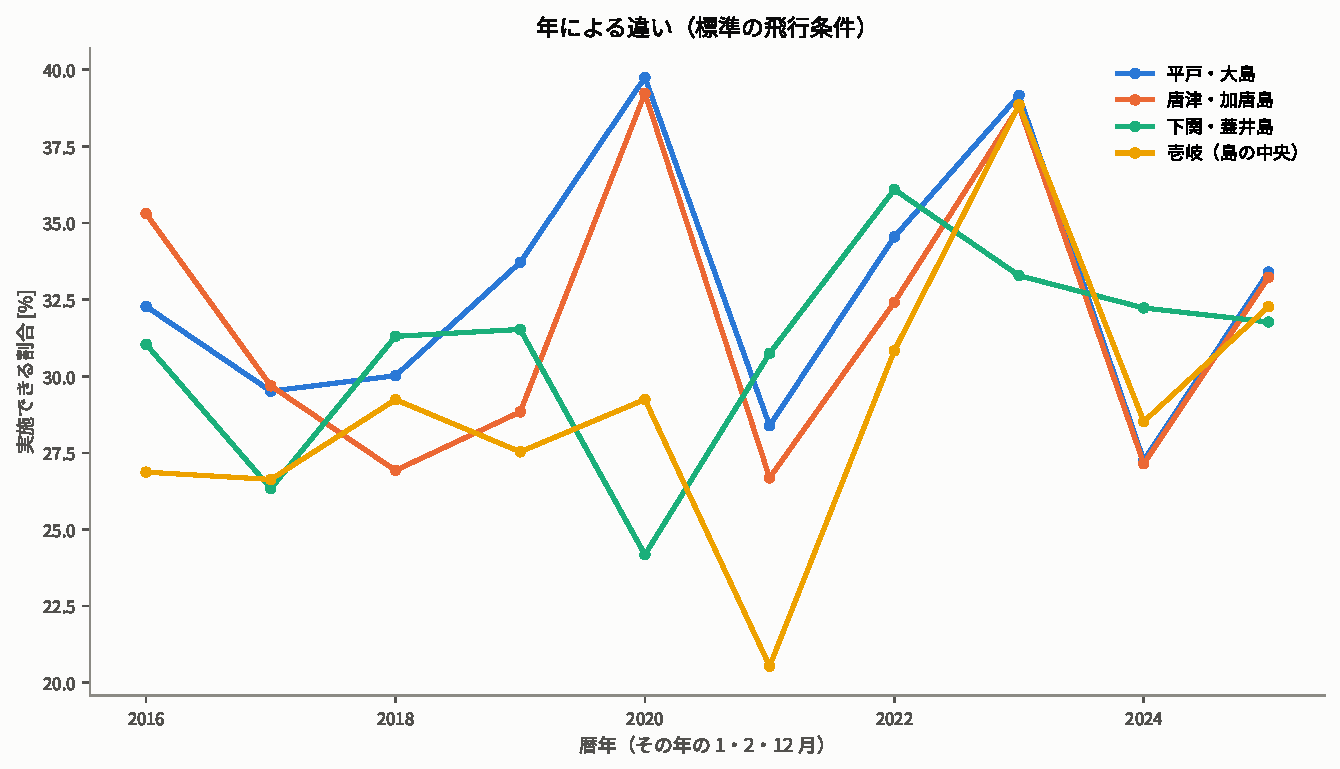
\includegraphics[width=\linewidth]{by_year.pdf}
\caption{年ごとの実施できる確率（その年の 1・2・12 月。冬のシーズンではなく暦年で分けた）。}
\label{fig:byyear}
\end{figure}
